\documentclass[11pt, a4paper]{article}

\usepackage[utf8]{inputenc}
\usepackage{geometry}
\geometry{a4paper, margin=1in}
\usepackage{graphicx}
\usepackage{hyperref}
\usepackage{xcolor}
\usepackage{float}
\usepackage{booktabs}
\usepackage{caption}
\usepackage{listings}
\usepackage{tcolorbox}
\usepackage{tabularx}
\usepackage{multirow}

% Setup links
\hypersetup{
    colorlinks=true,
    linkcolor=blue,
    filecolor=magenta,      
    urlcolor=blue,
    pdftitle={DS205.3 Technical Report},
}

% Code block styling
\definecolor{backcolour}{rgb}{0.95,0.95,0.92}
\lstset{
    backgroundcolor=\color{backcolour},   
    basicstyle=\ttfamily\footnotesize,
    breakatwhitespace=false,         
    breaklines=true,                 
    captionpos=b,                    
    keepspaces=true,                 
    showspaces=false,                
    showstringspaces=false,
    showtabs=false,                  
    tabsize=2,
    frame=single
}

\title{
    \vspace{-1.5cm}
    \textbf{DS205.3 -- Data Science with Python} \\
    \Large Technical Design \& Evaluation Report \\
    \large AI Startup Funding \& Investment Intelligence Assistant \\
    \normalsize \textit{A Retrieval-Augmented Generation (RAG) System}
}

\author{\textbf{Group Members:} Kisara, Dilusha, Savindi, Tharusha \\
\small \textbf{GitHub:} \url{https://github.com/Kisara00555/DS-in-Python}}
\date{\today}

\begin{document}

\maketitle

\hrule
\vspace{0.5cm}

% ---------------------------------------------------------
% SECTION I: PROBLEM STATEMENT
% ---------------------------------------------------------
\section{Problem Statement}

Large Language Models (LLMs) such as GPT-4, Llama, and Claude have demonstrated remarkable fluency in natural language understanding and generation. However, they suffer from two fundamental architectural limitations that make them unreliable for domain-specific knowledge work:

\subsection{Training Data Cutoffs}
LLMs are trained on static snapshots of internet data. For rapidly evolving domains like venture capital and AI startup funding, this means the model's knowledge becomes outdated within months. For example, a model trained in early 2025 would have no awareness of Q1 2026 VC funding totals, recent megadeals, or shifting investment patterns---precisely the kind of time-sensitive intelligence that investors, founders, and analysts need.

\subsection{Lack of Access to Private, Specialised Data}
Even if an LLM's training data were perfectly current, it has no access to private or niche documents---proprietary KPMG Venture Pulse reports, internal startup funding guides, or curated AI ecosystem analyses. These documents contain the granular, source-attributed data points (exact dollar figures, deal counts, regional breakdowns) that professionals require. An LLM asked about these topics will either refuse to answer or, worse, \textbf{hallucinate} plausible-sounding but fabricated statistics---a critical failure mode in financial contexts where accuracy is non-negotiable.

\subsection{Why a Standard LLM Is Insufficient}
When we prompted a standard LLM (Llama 3.1 8B) with the question \textit{"What was the total amount of VC funding raised globally in Q1 2026?"}, it either refused to answer (citing knowledge cutoff) or generated a fabricated figure. The correct answer---\textbf{\$330.9 billion}, sourced from the KPMG Private Enterprise Venture Pulse Q1 2026 report---can only be provided if the system has access to that specific document and can retrieve the relevant passage before generating its response.

\subsection{Our Solution: Retrieval-Augmented Generation (RAG)}
To bridge this gap, we built an RAG system that:
\begin{itemize}
    \item Ingests a curated corpus of \textbf{5 real-world PDF documents} covering AI funding, venture capital trends, and startup investment guides.
    \item Chunks, embeds, and stores these documents in a \textbf{persistent vector database} (ChromaDB).
    \item At query time, retrieves the most \textbf{semantically relevant passages} and feeds them as context to the LLM.
    \item Forces the LLM to generate answers \textbf{grounded exclusively in the retrieved evidence}, with source attribution.
\end{itemize}

This architecture eliminates both limitations: the system's knowledge is as current as the most recently ingested document, and it can access any private corpus---without retraining the model. Crucially, every answer includes a \textbf{traceability chain} showing exactly which source documents and pages influenced the response, enabling users to verify claims against the original evidence.

% ---------------------------------------------------------
% SECTION II: SYSTEM ARCHITECTURE & DESIGN
% ---------------------------------------------------------
\section{System Architecture \& Design}

\subsection{Modular Decomposition}
The system follows a strict modular Object-Oriented design, decomposed into five packages that each own a single responsibility. All inter-component communication uses \textbf{Dependency Injection} via abstract base classes (ABCs), making every component independently testable and swappable.

\begin{lstlisting}[language=bash, caption={System Architecture Data Flow}]
data/pdfs/ (PDF Corpus)
       | DocumentPage[]
       v
ingestion/pdf_loader.py (PyMuPDFLoader -> BaseLoader ABC)
       | DocumentPage[]
       v
ingestion/chunker.py (SlidingWindowChunker -> BaseChunker ABC)
       | TextChunk[]
       v
vectorstore/embedder.py (LocalEmbedder -> BaseEmbedder ABC)
       | float[][] (embedding vectors)
       v
vectorstore/store.py (ChromaVectorStore -> BaseVectorStore ABC)
       |
User Query ---> agent/retriever.py (Query expansion -> k-NN)
       | RetrievalTrace (chunks + metadata)
       v
agent/generator.py (Groq API Llama 3.1 8B)
       | GenerationResult (answer + trace)
       v
evaluation/evaluator.py (RAG Triad + Deterministic Metrics)
\end{lstlisting}

\subsection{Key Design Decisions}

\begin{tcolorbox}[colback=blue!5,colframe=blue!40!black,title=Embedding Model: all-MiniLM-L6-v2 (Local)]
We chose a local sentence-transformer model over a cloud-based embedding API for three reasons: (1) zero API quota or rate limits during batch ingestion of hundreds of chunks, (2) fully offline operation, and (3) 384-dimensional vectors provide excellent retrieval quality for our domain while keeping storage compact.
\end{tcolorbox}

\begin{tcolorbox}[colback=green!5,colframe=green!40!black,title=Chunking Strategy: Sliding Window (800/150)]
After testing fixed-size, recursive, and sentence-based chunking, we chose a sliding window approach with 800-character chunks and 150-character overlap. The overlap ensures that concepts spanning chunk boundaries are captured in at least one chunk. We use sentence-aware boundary detection to avoid splitting mid-sentence.
\end{tcolorbox}

\begin{tcolorbox}[colback=yellow!5,colframe=yellow!40!black,title=Vector Store \& LLM Selection]
\textbf{ChromaDB} was selected for its persistent on-disk storage and HNSW indexing for fast approximate nearest-neighbour search. For the LLM, we use \textbf{Llama 3.1 8B via Groq} for sub-second response times and strong instruction-following capabilities.
\end{tcolorbox}

% ---------------------------------------------------------
% SECTION III: IMPLEMENTATION & TRACEABILITY
% ---------------------------------------------------------
\section{Implementation \& Traceability}

\subsection{The Agentic Loop}
The core of the system is the \textbf{Agentic Loop} implemented in \texttt{rag\_agent.py}, which orchestrates the full pipeline in three steps:

\textbf{Step 1: Retrieve.} The Retriever first performs \textbf{query expansion}---using the LLM to generate 3 semantically diverse sub-queries from the original question. Each sub-query is embedded and searched against the vector store independently. Results are merged, deduplicated by chunk ID, and the top-5 chunks are returned.

\textbf{Step 2: Trace.} Before generating an answer, the system constructs a complete \textbf{Retrieval Trace} showing the original query, expanded sub-queries, each retrieved chunk (with source filename, page number, similarity score), and a preview of the chunk text. This provides an auditable record of exactly what context influenced the LLM's answer.

\textbf{Step 3: Generate.} The retrieved chunks are formatted into a numbered context block and passed to the LLM alongside the user's question. The prompt explicitly instructs the LLM to only use information from the provided context and to cite sources using \texttt{(Source: filename, Page X)} format.

\subsection{Retrieval vs. Generation: A Concrete Example}
\textbf{Question:} \textit{"What was the total amount of VC funding raised globally in Q1 2026?"}

\begin{lstlisting}[caption={Example of Retrieved Chunks and Grounded Generation}]
[Retrieved Chunk 1] kpmg-venture-pulse-q1-26-global-report.pdf | Page 7
  "VC-backed companies raised $330.9 billion across 7,505 deals in Q1'26..."

[Generated Answer]
"In Q1 2026, VC-backed companies raised a total of $330.9 billion globally across 7,505 deals (Source: kpmg-venture-pulse-q1-26-global-report.pdf, Page 7)..."
\end{lstlisting}
The answer is \textbf{grounded}---every claim traces back to a specific chunk and page.

% ---------------------------------------------------------
% SECTION IV: EMPIRICAL EVALUATION
% ---------------------------------------------------------
\section{Empirical Evaluation}

Quality is measured using a \textbf{dual-methodology} approach combining LLM-as-Judge scoring (TruEra RAG Triad) and deterministic metrics against 12 ground-truth questions.

\subsection{Aggregate Results}
\begin{table}[H]
\centering
\begin{tabular}{lc}
\toprule
\textbf{Metric} & \textbf{Average Score} \\
\midrule
Context Relevance (LLM-as-Judge) & 70.83\% \\
Faithfulness (LLM-as-Judge) & 80.00\% \\
Answer Relevance (LLM-as-Judge) & 92.50\% \\
\textbf{RAG Score (Harmonic Mean)} & \textbf{79.47\%} \\
\midrule
Precision (Keyword Specificity) & 53.59\% \\
Recall (Knowledge Coverage) & 63.61\% \\
F1 Score & 58.13\% \\
Cosine Similarity (Semantic Match) & 80.16\% \\
\bottomrule
\end{tabular}
\caption{Aggregate evaluation metrics across 12 ground-truth questions.}
\end{table}

\subsection{Analysis of Results}
\begin{itemize}
    \item \textbf{Answer Relevance is consistently the strongest metric (92.5\%)}, indicating the LLM is highly capable at generating on-topic responses when given relevant context.
    \item \textbf{Context Relevance is the weakest RAG Triad dimension (70.8\%)}, particularly for conceptual questions. The system must partially infer from scattered mentions across multiple documents.
    \item \textbf{Faithfulness at 80.0\%} confirms low hallucination rates. 
    \item \textbf{Cosine Similarity (80.16\%)} provides a complementary view to keyword metrics. The system captured the semantic intent of answers even when specific terminology differed from the ground truth.
\end{itemize}

\subsection{Evaluation Visualisations}
% Ensure the user has the images in the correct path or modifies this path.
\begin{figure}[H]
    \centering
    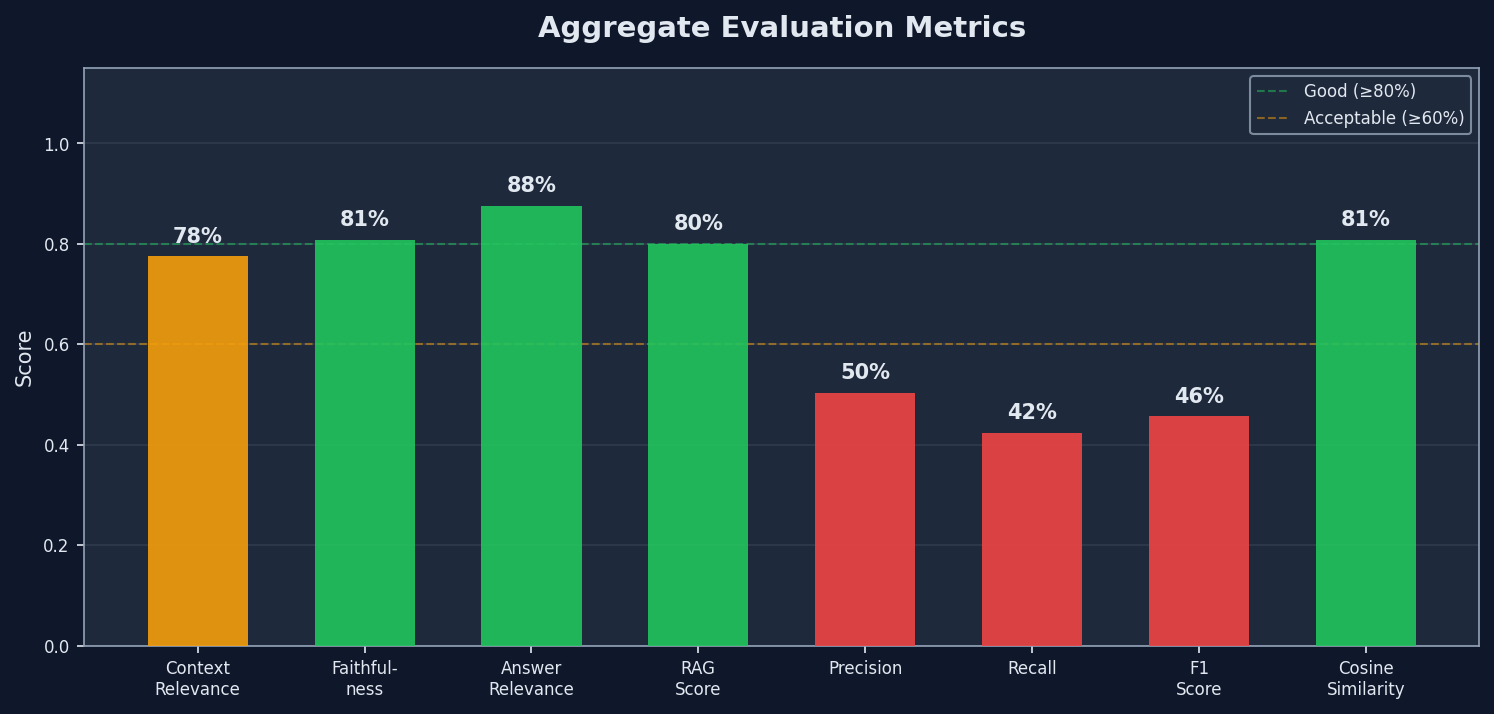
\includegraphics[width=0.8\textwidth]{data/evaluation/chart_summary.png}
    \caption{Aggregate bar chart showing all 8 metric averages with Good and Acceptable threshold lines.}
\end{figure}

\begin{figure}[H]
    \centering
    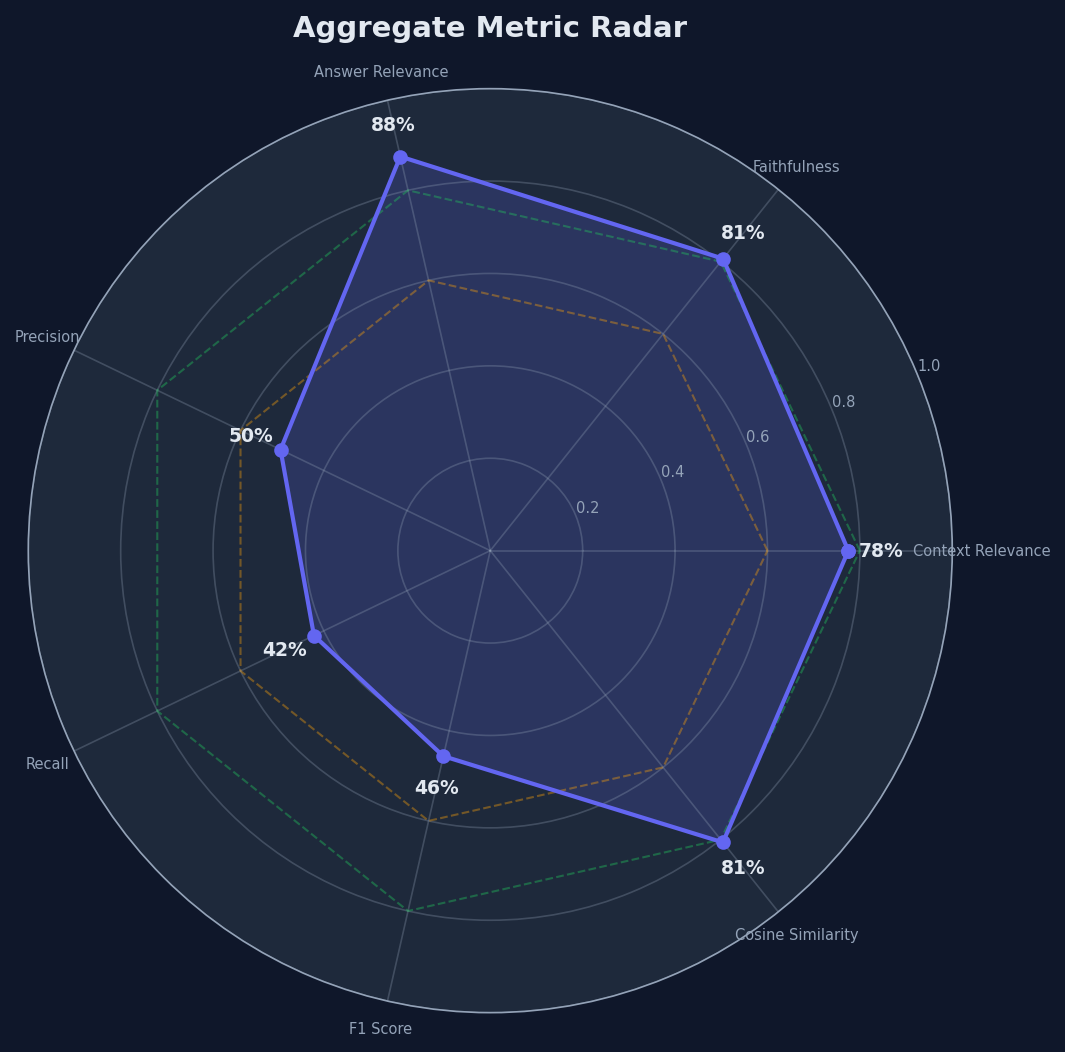
\includegraphics[width=0.8\textwidth]{data/evaluation/chart_radar.png}
    \caption{Spider/radar chart showing the metric profile.}
\end{figure}

% ---------------------------------------------------------
% SECTION V: PERSONAL REFLECTION
% ---------------------------------------------------------
\section{Personal Reflection}

\subsection{From Procedural Scripting to Object-Oriented AI Development}
The transition from writing procedural Python scripts to building a modular, object-oriented AI system was the most significant learning experience of this module. Designing abstract base classes required us to think about \textit{interfaces} before \textit{implementations}. The Dependency Injection pattern meant we could swap embedding strategies without touching retrieval logic.

\subsection{Debugging RAG Systems is Non-Trivial}
Unlike traditional software where bugs produce clear errors, RAG failures are subtle: the system might retrieve plausible but irrelevant chunks, or the LLM might generate a fluent but unfaithful answer. Building the traceability system---printing every retrieved chunk before generation---was essential for diagnosing these issues.

\subsection{The Value of Evaluation-Driven Development}
Implementing the RAG Triad evaluation framework early fundamentally changed our workflow. Instead of subjectively assessing answers, we could run \texttt{python evaluate.py} after each change and see exactly how modifications affected aggregate scores. This empirical feedback loop made optimisation systematic.

% ---------------------------------------------------------
% SECTION VI: FUTURE WORK
% ---------------------------------------------------------
\section{Future Work}

\begin{itemize}
    \item \textbf{Reflection Step (Agentic Improvement):} Add a "reflection" agent that reviews the generated answer against the retrieved context before presenting it to the user. If hallucinations are detected, it triggers a second retrieval pass.
    \item \textbf{Multimodal Support:} Extracting and embedding visual elements (charts, tables) from VC reports using models like GPT-4V to improve coverage for data-rich documents.
    \item \textbf{Metadata-Based Re-Ranking:} Boosting chunks from more authoritative sources or more recent documents to improve Context Relevance scores.
    \item \textbf{Hybrid Search:} Combining dense vector search (all-MiniLM-L6-v2) with sparse keyword search (BM25) to improve recall for specific technical terms or exact figures.
\end{itemize}

% ---------------------------------------------------------
% REFERENCES
% ---------------------------------------------------------
\begin{thebibliography}{9}
\bibitem{kpmg} 
KPMG Private Enterprise (2026). \textit{Venture Pulse Q1 2026 — Global Analysis of Venture Funding}.
\bibitem{stanford} 
Stanford University (2026). \textit{AI Index Report 2026}.
\bibitem{pwc} 
PwC (2026). \textit{Global Business Ecosystems 2030}.
\bibitem{truera}
TruEra (2023). \textit{The RAG Triad: Measuring RAG Quality}. TruLens Documentation.
\bibitem{reimers}
Reimers, N. and Gurevych, I. (2019). \textit{Sentence-BERT: Sentence Embeddings using Siamese BERT-Networks}. ACL 2019.
\bibitem{lewis}
Lewis, P. et al. (2020). \textit{Retrieval-Augmented Generation for Knowledge-Intensive NLP Tasks}. NeurIPS 2020.
\end{thebibliography}

\end{document}
